\section{The sample complexity of SGD}
In this section, we focus on understanding the complexity of the SGD algorithm, i.e., how the number of total gradient steps \(n\) scales with the dimension \(d\) of the token embeddings, in the high-dimensional limit \(d\gg 1\); for simplicity of exposition, we focus on the case \(k=1\), but the same arguments can be repeated for each of the components of the output.  

\paragraph{No positional encoding ---} We first focus on the case without positional encoding: \(P=0\) implies that the only relevant sufficient statistic is \(m\). An analogy with single-index models for networks can be done: For single-index models, the \emph{information exponent} fully characterizes the sample complexity of the SGD algorithm \cite{arous2021online}. The definition can be generalized for sequential data.
\begin{definition}[Sequence Information Exponent (SIE)] \label{2506:def:sie}
    Given \(\vec{f}^\mathrm{SSI}_{\vec w_{\star}}(X)\) a sequence single-index model, let \(g\) be the function that acts on the local field \(\vec{z}_\star\), we define the \emph{sequence information exponent} as
    \[
        \text{SIE}(\vec{f}^\mathrm{SSI}_{\vec w_{\star}}(X)) \coloneqq
            \min \left\{
                \sum^L_{l=1}k_l > 0 \colon
                    \vec{k}\in\mathbb{N}^L,
                    \mathbb{E}_{\vec{z}\sim\mathcal{N}(0,I_L)}\left[
                        \left(\prod^L_{l=1}\mathrm{He}_{k_l}(z_l)\right)g(\vec{z})
                    \right] \neq 0
            \right\},
    \]
    where \(\mathrm{He}_k\) is the \(k\)-th order Hermite polynomial.
\end{definition}
In Appendix~\ref{2506:app:hermite-polynomials} we provide more details on Hermite polynomials.
Let us give some examples of SIE for different SSI models:
\begin{itemize}
    \item \(g(\vec{z}_\star) = z_{\star,1} + z_{\star,2} + \dots + z_{\star,L}\) has \(\text{SIE} = 1\);
    \item \(g(\vec{z}_\star) = z_{\star,1}z_{\star,2} = \mathrm{He}_1(z_{\star,1})\mathrm{He}_1(z_{\star,2})\) has \(\text{SIE} = 2\);
    \item \(g(\vec{z}_\star) = \mathrm{He}_1(z_{\star,1})\mathrm{He}_4(z_{\star,2})+\mathrm{He}_2(z_{\star,3})\mathrm{He}_2(z_{\star,4})\) has \(\text{SIE} = 4\);
    \item \(g(\vec{z}_\star) = \prod_{l=1}^L \mathrm{He}_{k_l}(z_{\star,l})\) has \(\text{SIE} = \sum_{l=1}^L k_l\).
\end{itemize}
The main feature of the information exponent is that it can be connected to the sample complexity of the SGD algorithm; we prove an equivalent result for the sequence information exponent.
\begin{theorem}[Informal] \label{2506:thm:sie}
    Let \(\vec{f}^\mathrm{SSI}_{\vec w_{\star}}(X)\) be a sequence single-index model, and let \(\text{SIE}\) be its sequence information exponent. If the model \(f_{\vec{w}}\) has a rich enough Hermite expansion, then the sample complexity of the SGD algorithm is
    \[
        t^+_\eta = \begin{cases}
            \mathcal{O}_L(d) & \text{if } \text{SIE} = 1 \\
            \mathcal{O}_L(d \log^2 d) & \text{if } \text{SIE} = 2 \\
            \mathcal{O}_L(d^{\text{SIE}-1}) & \text{if } \text{SIE} \ge 3 
        \end{cases}.
    \]
\end{theorem}
A formal statement of the Theorem and the proof are given in the Appendix~\ref{2506:app:proofs}. 

\begin{figure}
    \centering
    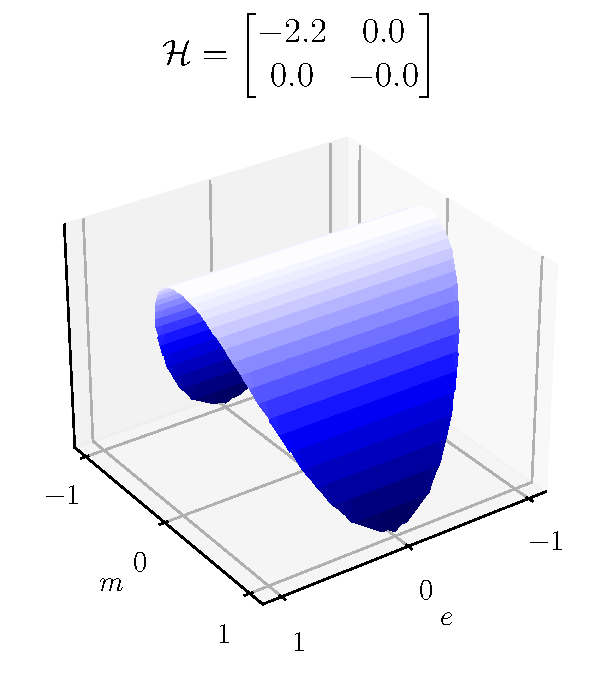
\includegraphics[width=0.49\textwidth]{figs/plot_surface/loss_surface_SIE2_peFalse}
    %
    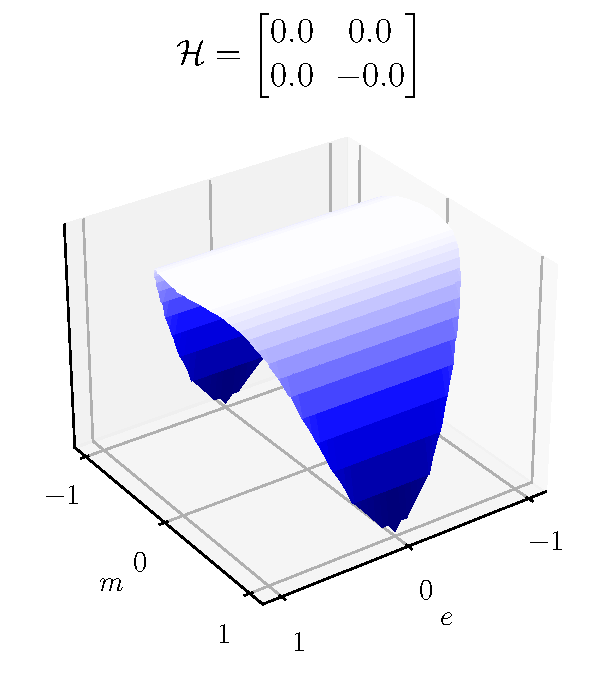
\includegraphics[width=0.49\textwidth]{figs/plot_surface/loss_surface_SIE4_peFalse}
    %
    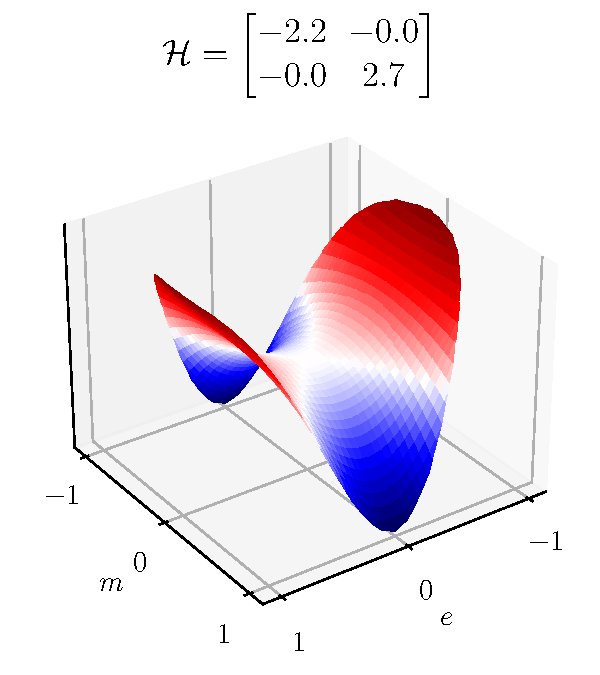
\includegraphics[width=0.49\textwidth]{figs/plot_surface/loss_surface_SIE2_peTrue}
    %
    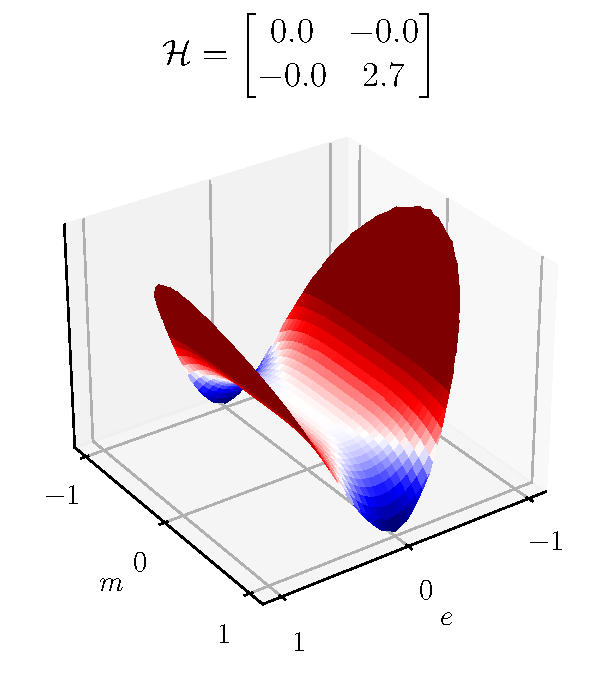
\includegraphics[width=0.49\textwidth]{figs/plot_surface/loss_surface_SIE4_peTrue}
    \caption{the landscape of the population risk, together with the hessian at initialization, for different values of the SIE and positional encoding.
    (left) \(g(\vec{z}_\star) = \mathrm{He}_2(\vec{z}_{\star,1}) + \mathrm{He}_2(\vec{z}_{\star,2})\): SIE=2, no positional encoding: null gradient, but non-null hessian;
    (center-left) SIE=4, no positional encoding: the first non-null term at initialization is at the 4th order;
    (center-right) \(g(\vec{z}_\star) = \mathrm{He}_4(\vec{z}_{\star,1}) + \mathrm{He}_4(\vec{z}_{\star,2})\): SIE=2, with positional encoding: again dynamic dominated by the hessian, but we have a positive curvature in the direction of \(e\);
    (right) SIE=4, with positional encoding: hessian is positive semidefinite, and the dynamic is again at 4th order in direction of \(e\).
    In all the examples \(L=2, P_1=-P_2, R = \Tr\).
    }
    \label{2506:fig:loss_surface}
\end{figure}
In Figure~\ref{2506:fig:loss_surface}, we show some examples of the population loss landscape for different values of the SIE. The SIE can also be interpreted as the first non-null order in Taylor expansion of the loss at the initialization point, and consequently the number of gradient steps needed to build up a weak correlation is higher. Figure~\ref{2506:fig:loss_surface} focuses on even SIE because the symmetry of Equation~\eqref{2506:eq:model-definition} restricts the possible targets to even functions; in the Appendix~\ref{2506:app:sie-extra} we discuss how to surpass this limitation, and we present settings with odd SIE. 


\paragraph{The effect of positional encoding ---}
Despite the fact that positional encoding only acts on the trained model, and not the target function, it changes the population loss, potentially changing the dynamic at initialization.
In particular, adding  positional encoding increase the expressivity of the model, and  can ultimately lead to faster weak-recovery of the SGD.
\begin{lemma}
    Let \(f_{\vec{w}}\) be a model with \(P=0\) that learns a target \(\vec{f}^\mathrm{SSI}_{\vec w_{\star}}(X)\) with a given \(\mathrm{SIE}\). If we add a positional encoding \(P\) to the model, and let \(\mathrm{SIE}_\mathrm{positional}\) be the SIE of the new model, then
    \[
        \mathrm{SIE}_\mathrm{positional} \le \mathrm{SIE}.
    \]
\end{lemma}
In other words, the positional encoding can only decrease the SIE of the model, thus the sample complexity of the SGD algorithm could be reduced. The proof of this lemma is given in the Appendix~\ref{2506:app:proofs}.
\begin{figure}
    
    \centering
    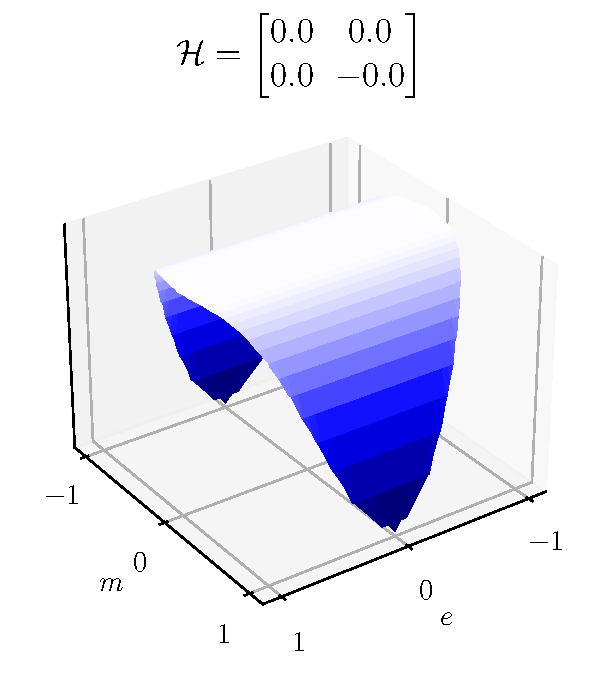
\includegraphics[width=0.49\textwidth]{figs/plot_surface/loss_surface_SIEPE_peFalse}
    %
    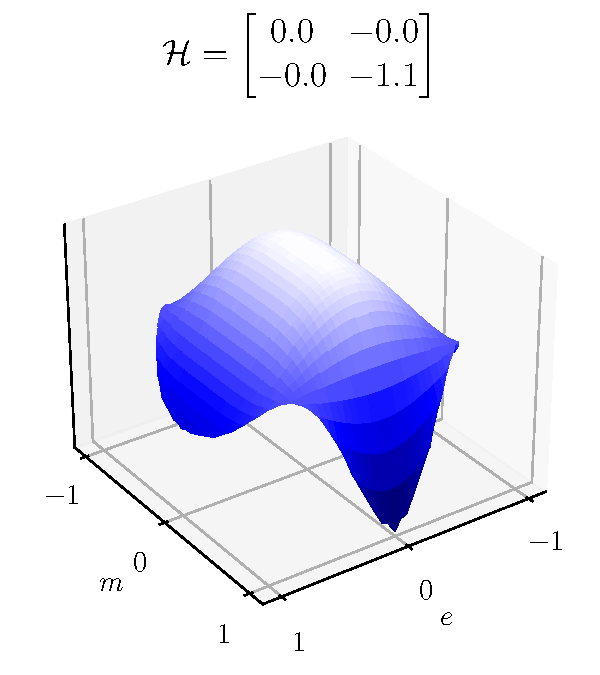
\includegraphics[width=0.49\textwidth]{figs/plot_surface/loss_surface_SIEPE_peTrue}
    \caption{Population loss landscape for \(P=0\) (left) and \(P\neq 0\) (right). Example of a case where \({\rm SIE}=4\), while \({\rm SIE}_\mathrm{positional}=2\). Target: \(g(\vec{z}_\star) = \sfrac43 + \mathrm{He}_4(z_1) + 2\mathrm{He}_4(z_{\star,2})\), \(P_1=-P_2\), \(R = \Tr\). 
    }
    \label{2506:fig:loss_surface_pe}
    % 
\end{figure}
In the right part of Figure~\ref{2506:fig:loss_surface_pe}, we present an example  where adding the positional encoding can improve the sample complexity of the SGD algorithm. The left part of Figure~\ref{2506:fig:loss_surface_pe} shows that the population loss landscape at initialization is flat, and the hessian is null: the first non-null term in the Taylor expansion is at order 4, hence the SIE is 4. The right part of Figure~\ref{2506:fig:loss_surface_pe} shows instead that when we add the positional encoding, a non-null term appears at order 2, and \(\mathrm{SIE}_\mathrm{positional} = 2\). 
Note that the position of the global minima is not affected by the positional encoding, but SGD can converge to the new local minima; more discussion on this point is given in Section~\ref{2506:sec:positional_encoding}.
In contrast, the right part of Figure~\ref{2506:fig:loss_surface} shows that the positional encoding is not necessarily beneficial: there are cases for which the loss landscape changes, but not the sample complexity.
